\documentclass[polish,polish,a4paper,12pt]{article}

\usepackage{amsmath} %koniecznie
\usepackage{amssymb,amsfonts,amsthm} %dodatkowo
\usepackage[T1]{fontenc}
\usepackage[utf8]{inputenc}
\usepackage{babel}
\usepackage{pslatex}
\usepackage{graphicx}
\usepackage{anysize}
\usepackage{titling}
\graphicspath{ {./images/} }
\marginsize{2.5cm}{2.5cm}{3cm}{3cm}

\setlength{\droptitle}{-2cm}
\title{Symulator kontroli pH z regulacją stężenia kwasu}
\date{}
\author{Mikołaj Kiszka, Katarzyna Jaromirska, Łukasz Grobelny}
\begin{document}
	
	\maketitle
	\vspace{-4\baselineskip}
	
	\section{Opis symulatora}
	
	Zaprojektowany przez nas symulator obejmuje pojemnik z \textbf{dwoma dopływami} oraz \textbf{jednym odpływem}. 
	
	Jeden z dopływów o stałym natężeniu dopływu wprowadza do zbiornika kwas o zmierzonym, stałym bądź oscylującym wokół pewnej wartości stężeniu. Drugim dopływem wlewa się do zbiornika, z regulowanym przez nas natężeniem, kwas o określonym stężeniu. Równocześnie pojemnik posiada otwór przez, który stale następuje wypływ kwasu znajdującego się w pojemniku. Kwas jest wybierany przez użytkownika spośród 10 dostępnych kwasów.
	
	Zaprojektowany symulator ma na celu przez regulację drugiego dopływu dążenie do zadanego pH roztworu w zbiorniku
	
	\section{Teoria oraz zastosowane równania i przekształcenia}
	
	Po określeniu stężeń obu dopływów oraz zakładając całkowite mieszanie z bilansu masy całkowitej można wyprowadzić wzory różnicowe opisujące zmianę objętości cieczy $V$ oraz jej stężenia w pojemniku $c$:
	
	\begin{equation}
		\begin{cases}
			\frac{dV(t)}{dt} = Q_{d_{1}}(t) + Q_{d_{2}}(t) - Q_{o}(t) \\
			\frac{dc(t)}{dt} = \frac{1}{V(t)} \cdot \left(Q_{d_{1}}(t) \left(c_{d_{1}}(t) - c(t)\right) + Q_{d_{2}}(t)\left(c_{d_{2}}(t) - c(t)\right)\right)		
		\end{cases}
	\end{equation}
	
	z czego wynikają bezpośrednio rekurencyjne rozwiązania równań różnicowych dla wysokości oraz stężęnia cieczy:
	
	\begin{equation}
		\begin{cases}
			h(0) = h_{0}\\
			h(n+1) =\frac{1}{A} \cdot T_{p} \cdot \left(Q_{d_{1}}(n) + Q_{d_{2}}(n) - Q_{0}(n)\right) + h(n)\\
			c(0) = c_{0}\\
			c(n+1) = \frac{1}{A \cdot  h(n)} \cdot T_{p} \cdot \left(Q_{d_{1}}(n)\left(c_{d_{1}}(n) - c(n)\right) + Q_{d_{2}}(n)\left(c_{d_{2}}(n) - c(n)\right)\right)
		\end{cases}
	\end{equation}
	
	{\small V - objętość substancji w zbiorniku [$m^3$], \hspace{1em}h - poziom substancji w zbiorniku [$m$], \hspace{1em}A - pole powierzchni przekroju poprzecznego zbiornika [$m^2$], \hspace{1em}c - stężenie kwasu [\%], \hspace{1em}$Q_{d_{1}}$ - natężenie dopływu regulowanego [$m^3/s$], \hspace{1em}$Q_{d_{2}}$ - natężenie dopływu nieregulowanego [$m^3/s$], \hspace{1em} $Q_0$ - natężenie odpływu [$m^3/s$] ($Q_0(t) = \beta \sqrt{h(t)}$, gdzie $\beta$ - współczynnik wypływu [$m^{5/2}/s$]),\hspace{1em}$c_{d_{1}}$ - stężenie kwasu w dopływie regulowanym [\%], \hspace{1em}$c_{d_{2}}$ - stężenie kwasy w dopływie nieregulowanym [\%], \hspace{1em}$T_p$ - okres próbkowania [s]}
	
	Przedstawione wzory pozwalają wyznaczyć zmianę wysokości oraz stężenia procentowego kwasu w zależności od zadanych stężeń oraz natężeń dopływów. Z tego powodu zmienną docelową powinno być w tym przypadku stężenie procentowe kwasu w pojemniku.
	
	Jednakże, jak zaznaczyliśmy wyżej, naszym celem jest zaprojektowanie symulatora dążącego do określonego pH, nie stężenia procentowego. Potrzebne jest zatem wyznaczenie stężenia procentowego jako funkcji pH, co wiąże się z kolei z wyznaczeniem wzorów na pH roztworu w zależności od jego stężenia molowego (a także w drugą stronę) oraz znalezienie związku między stężeniem molowym oraz procentowym.
	
	W symulatorze wprowadziliśmy do wyboru tylko kwasy jedno, dwu i trzyprotonowe, a więc dla takich zostaną wyprowadzone powyższe zależności:
	
	\subsection{Zależność pH od stężenia molowego (i wzajemnie)}
	
	Stałe kwasowe dysocjacji $K_a$ są stałymi tabelowymi
	\begin{enumerate}
		\item Kwasy jednoprotonowe - $HX$
		\begin{equation*}
			HX \rightleftarrows H^+ + X^- \hspace{4em}K_{a_1} = \frac{|H^+||X^-|}{|HX|}
		\end{equation*}
		
		\begin{equation*}
			|H^+| = |X^-| = x \hspace{2em} |HX| = c-x \text{, c - stężenie molowe}
		\end{equation*}
		
		\begin{equation*}
			K_{a_1} = \frac{x^2}{c-x}
		\end{equation*}
		
		Po przekształceniu otrzymujemy równania:
		
		\begin{equation*}
			|H^+| = \frac{-K_{a_1} + \sqrt{4cK_{a_1} + K_{a_1}^2}}{2}
		\end{equation*}
		
		\begin{equation*}
			c = \frac{|H^+|^2+K_{a_1}|H^+|}{K_{a_1}}
		\end{equation*}
		
		\begin{equation*}
			\text{gdzie } pH = -\log |H^+| \text{ oraz } |H^+| = 10^{-pH}
		\end{equation*}
		
		\item Kwasy dwuprotonowe - $H_2X$
		\begin{equation*}
			H_2X \rightleftarrows H^+ + HX^- \hspace{4em} K_{a_1} = \frac{|H^+||HX^-|}{|H_2X|}
		\end{equation*}
		
		\begin{equation*}
			HX^- \rightleftarrows H^+ + X^{2-} \hspace{4em} K_{a_2} = \frac{|H^+||X^{2-}|}{|HX^-|}
		\end{equation*}
		
		Korzystając ze stężenia molowego kwasu oraz reguły elektroobojętności można zapisać:
		
		\begin{equation*}
			\begin{cases}
				c = |H_2X| + |HX^-| + |X^{2-}|\\
				|H^+| = |HX^-| + 2|X^{2-}| + |OH^-|
			\end{cases}
		\end{equation*}
		
		Wykluczenie bardzo małych stężeń (co wprowadziliśmy w postaci ograniczeń do symulatora) pozwala założyć:
		
		\begin{equation*}
			pH \leqslant 5 \Rightarrow |H^+| \gg |OH^-| \Rightarrow |H^+| - |OH^-| \approx |H^+|
		\end{equation*}
		
		a więc drugie równanie przyjmuje postać:
		
		\begin{equation*}
			|H^+| = |HX^-| + 2|X^{2-}|
		\end{equation*}
		
		Korzystając ze stałych dysocjacji $K_a$ można wyznaczyć równania:
		
		\begin{equation*}
			\begin{cases}
				c = \frac{|H^+||HX^-|}{K_{a_1}} + |HX^-| + \frac{K_{a_2}|HX^-|}{|H^+|}\\
				|H^+| = |HX^-| + \frac{2K_{a_2}|HX^-|}{|H^+}
			\end{cases}
		\end{equation*}
		
		Podzielenie obu równań przez $|HX^-|$, następnie podzielenie równań przez siebie oraz przekształcenie równania pozwala otrzymać:
		
		\begin{equation*}
			|H^+|^3 + K_{a_1}|H^+|^2 + \left(K_{a_1}K_{a_2} - cK_{a_1}\right)|H^+| - 2cK_{a_1}K_{a_2} = 0
		\end{equation*}
		
		\begin{center}
			(wystarczy znaleźć dodatni pierwiastek równania)
		\end{center}
		
		oraz:
		
		\begin{equation*}
			c = \frac{|H^+|^3 + K_{a_1}|H^+|^2 + K_{a_1}K_{a_2} |H^+|}{K_{a_1}|H^+| + 2K_{a_1}K_{a_2}}
		\end{equation*}
		
		\begin{equation*}
			\text{gdzie } pH = -\log |H^+| \text{ oraz } |H^+| = 10^{-pH}
		\end{equation*}
		
		\item Kwasy trzyprotonowe - $H_3X$
		
		\begin{equation*}
			H_3X \rightleftarrows H^+ + H_2X^- \hspace{4em} K_{a_1} = \frac{|H^+||H_2X^-|}{|H_3X|}
		\end{equation*}
		
		\begin{equation*}
			H_2X^- \rightleftarrows H^+ + HX^{2-} \hspace{4em} K_{a_2} = \frac{|H^+||HX^{2-}|}{|H_2X^-|}
		\end{equation*}
		
		\begin{equation*}
			HX^{2-} \rightleftarrows H^+ + X^{3-} \hspace{4em} K_{a_3} = \frac{|H^+||X^{3-}|}{|HX^{2-}|}
		\end{equation*}
		
		Korzystając ze stężenia molowego kwasu oraz reguły elektroobojętności można zapisać:
		
		\begin{equation*}
			\begin{cases}
				c = |H_3X| + |H_2X^-| + |HX^{2-}| + |X^{3-}|\\
				|H^+| =|H_2X^-| + 2|HX^{2-}| + 3|X^{3-}| + |OH^-|
			\end{cases}
		\end{equation*}
		
		Podobne do obliczeń dla kwasu dwuprotonowego założenie ($pH \leqslant 5$) oraz podobne przekształcenia pozwalają otrzymać:
		
		\begin{equation*}
			\begin{gathered}
				|H^+|^4 + K_{a_1}|H^+|^3 + \left(K_{a_1}K_{a_2} - cK_{a_1}\right)|H^+|^2 + \\
				\left(K_{a_1}K_{a_2}K_{a_3} - 2cK_{a_1}K_{a_2}\right)|H^+| - 3cK_{a_1}K_{a_2}K_{a_3} = 0
			\end{gathered}
		\end{equation*}
		
		\begin{center}
			(wystarczy znaleźć dodatni pierwiastek równania)
		\end{center}
		
		\begin{equation*}
			c = \frac{|H^+|^4 + K_{a_1}|H^+|^3 + K_{a_1}K_{a_2}|H^+|^2 + K_{a_1}K_{a_2}K_{a_3}|H^+|}{K_{a_1}|H^+|^2 + 2K_{a_1}K_{a_2}|H^+| + 3K_{a_1}K_{a_2}K_{a_3}}
		\end{equation*}
		
		\begin{equation*}
			\text{gdzie } pH = -\log |H^+| \text{ oraz } |H^+| = 10^{-pH}
		\end{equation*}
	\end{enumerate}
	
	\subsection{Zależność między stężeniem procentowym i stężeniem molowym}
	
	Zadane w obu dopływach stężenia, a także stężenie w opisanym wyżej równaniu różnicowym, jest stężeniem procentowym. Natomiast opisywane w poprzednim podpunkcie zależności wymagają użycia stężenia molowego.
	
	Wymagana jest więc w chwili wyboru zadanego pH, zamiana stężenia molowego na procentowe oraz w każdej iteracji zamiana stężenia procentowego na molowe w celu wyznaczenia aktualnego pH roztworu.
	
	Wyliczenie stężenia molowego z procentowego oraz w drugą stronę wymaga znajomości wartości gęstości roztworu. Niestety nie istnieje prosta zależność między tymi wartościami. Korzystając jednak ze źródeł ''Preparatyka Organiczna'', A.I.Vogel oraz ''The Engineering \mbox{ToolBox} (2017), Densities of Aqueous Solutions of Organic Acids'' znaleźliśmy gęstości roztworów wodnych kwasów dla danych stężeń procentowych oraz dla danego stężenia molowego (bezpośrednio lub wyliczonego z rozpuszczalności). Przybliżyliśmy więc te wartości do funkcji wielomianowych odpowiednich rzędów, aby jak najbardziej przybliżyć gęstość dla dowolnej wartości stężęnia procentowego lub molowego, co pokazano na poniższym przykładzie dla kwasu azotowego (V) - $HNO_3$.
	
	\begin{center}
		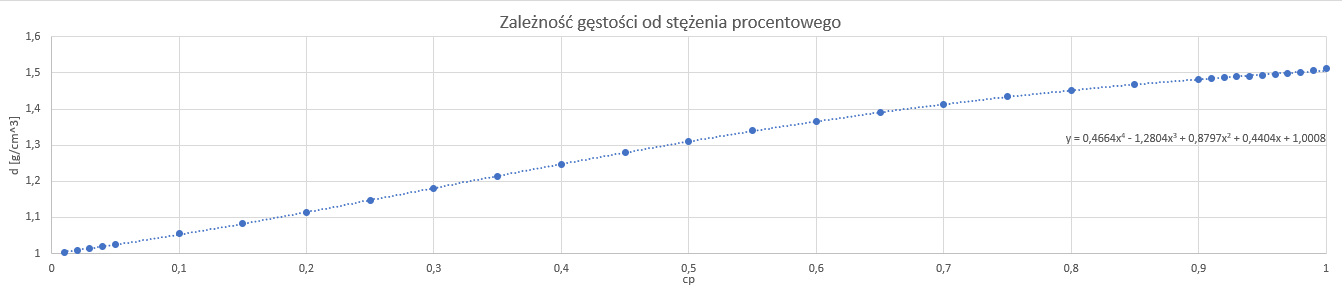
\includegraphics[scale=0.45]{1}\\
		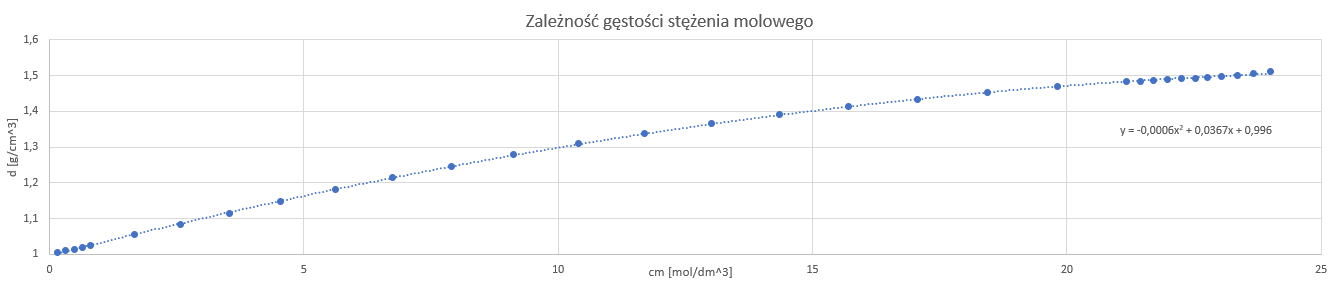
\includegraphics[scale=0.45]{2}\\
	\end{center}
	
	Z wyznaczonych funkcji wielomianowych można wyliczyć gęstość substancji dla dowolnego stężenia procentowego i molowego.
	
	Posiadając wartość gęstości można wyliczyć stężenie procentowe oraz molowe ze wzorów:
	
	\begin{equation*}
		c_p = \frac{c_mM}{1000 \cdot d}
	\end{equation*}
	
	\begin{equation*}
		c_m = \frac{1000 \cdot c_p d}{M}
	\end{equation*}
	
	{\small $c_p$ - stężęnie procentowe [\%], \hspace{1em} $c_m$ - stężenie molowe [$mol/dm^3$], \hspace{1em} M - masa molowa substancji [g/mol], \hspace{1em} d - gęstość [$g/cm^3$]}
	
	\section{Algorytm sterowania}
	
	W symulacji zastosowaliśmy dwa rodzaje regulatorów do wyboru przez użytkownika:
	
	\begin{enumerate}
		\item Regulator typu PI
		\begin{equation*}
			u(n) = k_p\left[e(n) + \frac{T_p}{T_i}\sum_{k=0}^{n}e(k)\right]
		\end{equation*}
		\item Regulator typu PID
		\begin{equation*}
			u(n) = k_p\left[e(n) + \frac{T_p}{T_i}\sum_{k=0}^{n}e(k) + \frac{T_d}{T_p}\Delta e(n)\right]
		\end{equation*}
		\begin{center}
			\small(Regulator typu PI można więc otrzymać, gdy $T_d = 0$)
		\end{center}
	\end{enumerate}
	
	\small{u - sygnał sterowania (napięcie) [V], $k_p$ - wzmocnienie regulatora, $T_p$ - okres próbkowania [s], $T_i$ - czas zdwojenia [s], $T_d$ - czas wyprzedzenia [s], e - uchyb regulacji}
	
	Wyliczony sygnał sterowania pozwala wyznaczyć natężenie dopływu, którym sterujemy w tym symulatorze, zgodnie ze wzorem:
	
	\begin{equation*}
		Q_{d_{1}}(n) = \frac{Q_{{d_{1}}_{max}} - Q_{{d_{1}}_{min}}}{u_{max} - u_{min}}\left(u(n) - u_{min}\right) + Q_{{d_{1}}_{min}}
	\end{equation*}
	
	\section{Nieuwzględnione zakłócenia i błędy}
	
	Zaprojektowany regulator nie jest skomplikowany, co wynika z wielu założonych uproszczeń, między innymi:
	
	\begin{enumerate}
		\item [--] założenie całkowitego wymieszania roztworu w pojemniku
		\item [--] założenie stałej temperatury (a więc założenie, że rozcieńczaniu i zatężaniu kwasu nie towarzyszy zmiana temperatury oraz że stałe dysocjacji $K_a$ są stałe)
		\item [--] założenie, że wysokoprocentowe kwasy są nieżrące a pojemnik niezniszczalny
		\item [--] założenie natychmiastowego wyrównania się wysokości roztworu
		\item [--] założenie stałego ciśnienia w pojemniku oraz dopływach
	\end{enumerate}
	
	\section{Przykładowe wykresy}
	
	\begin{center}
		\textbf{Pierwsze trzy wykresy przedstawiają wpływ rodzaju zakłócenia (mocnego i słabego) na wyniki.}\\
		\hspace{0em}\\
		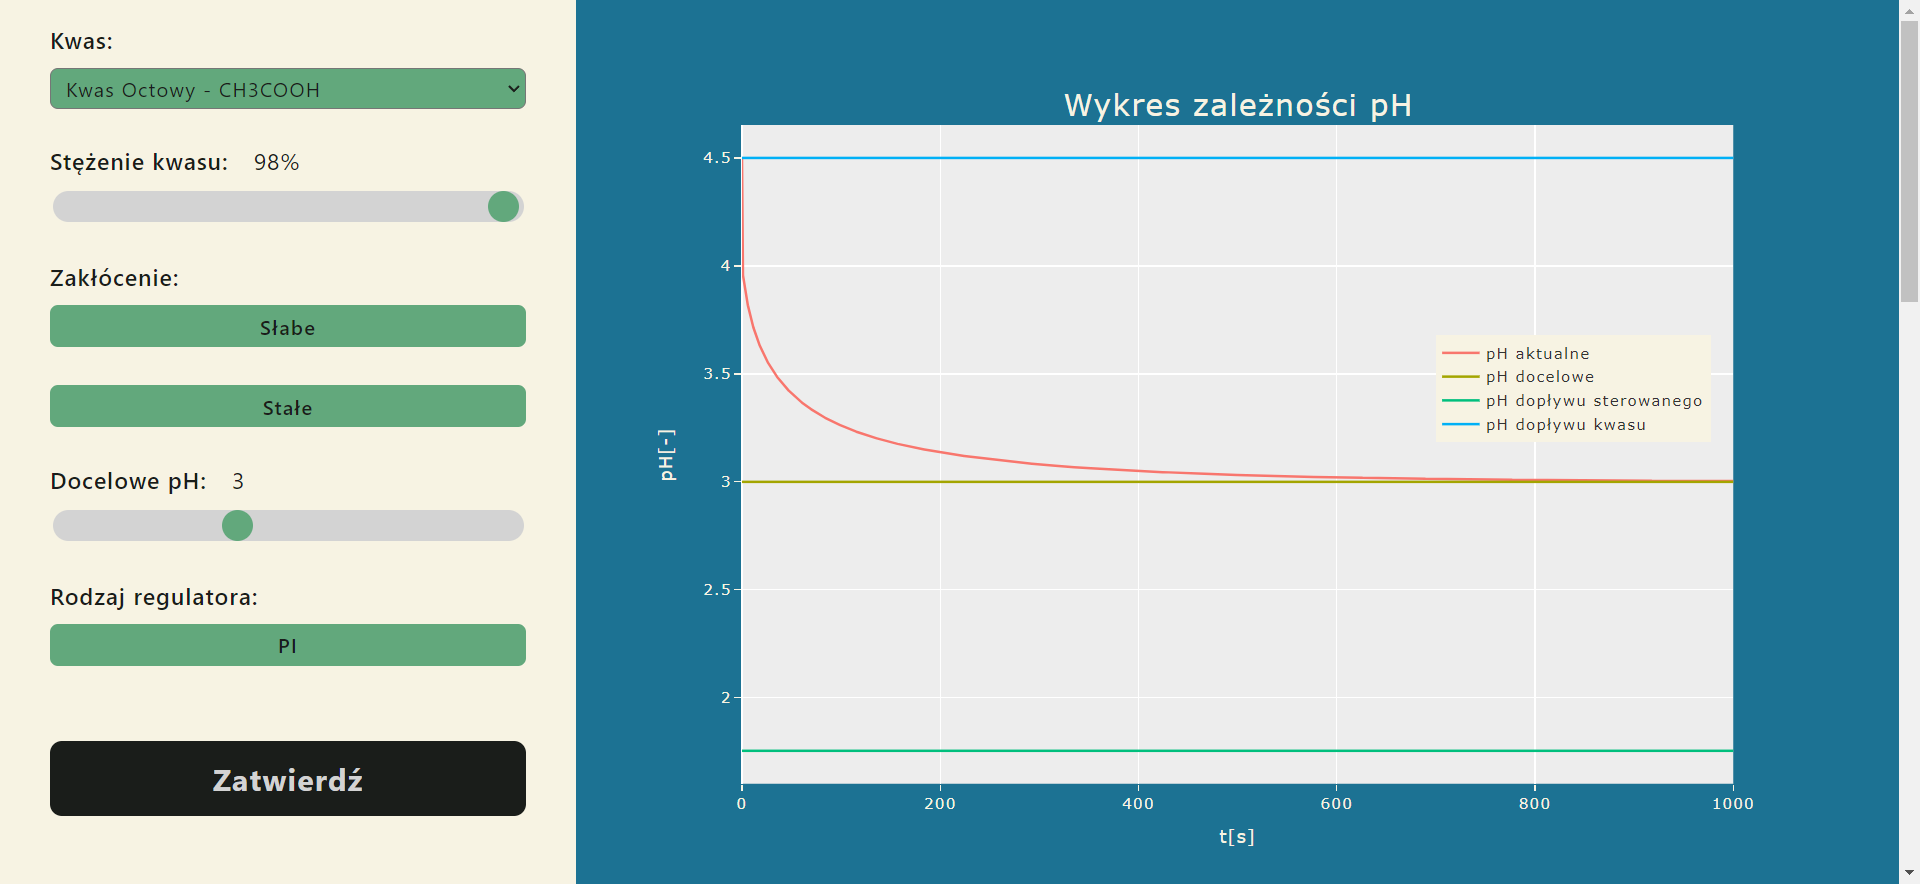
\includegraphics[scale=0.4]{octowy_98_3}\\
		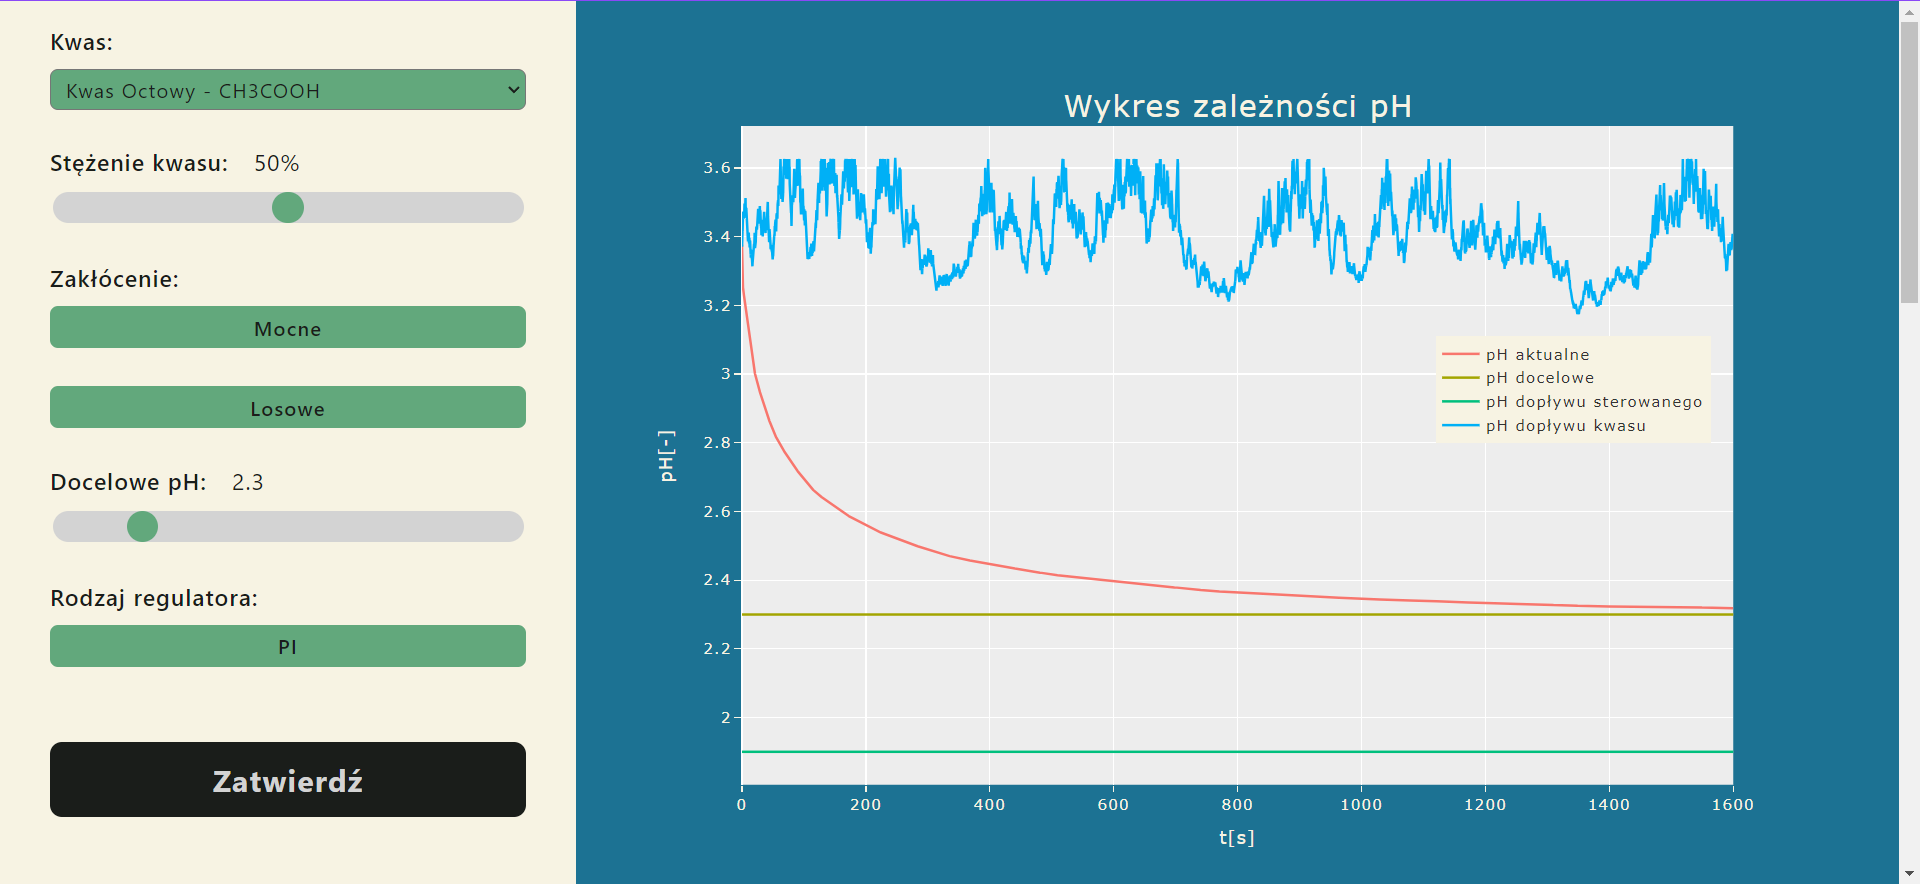
\includegraphics[scale=0.4]{octowy_50_2_3_losowe}\\
		\hspace{0em}\\
		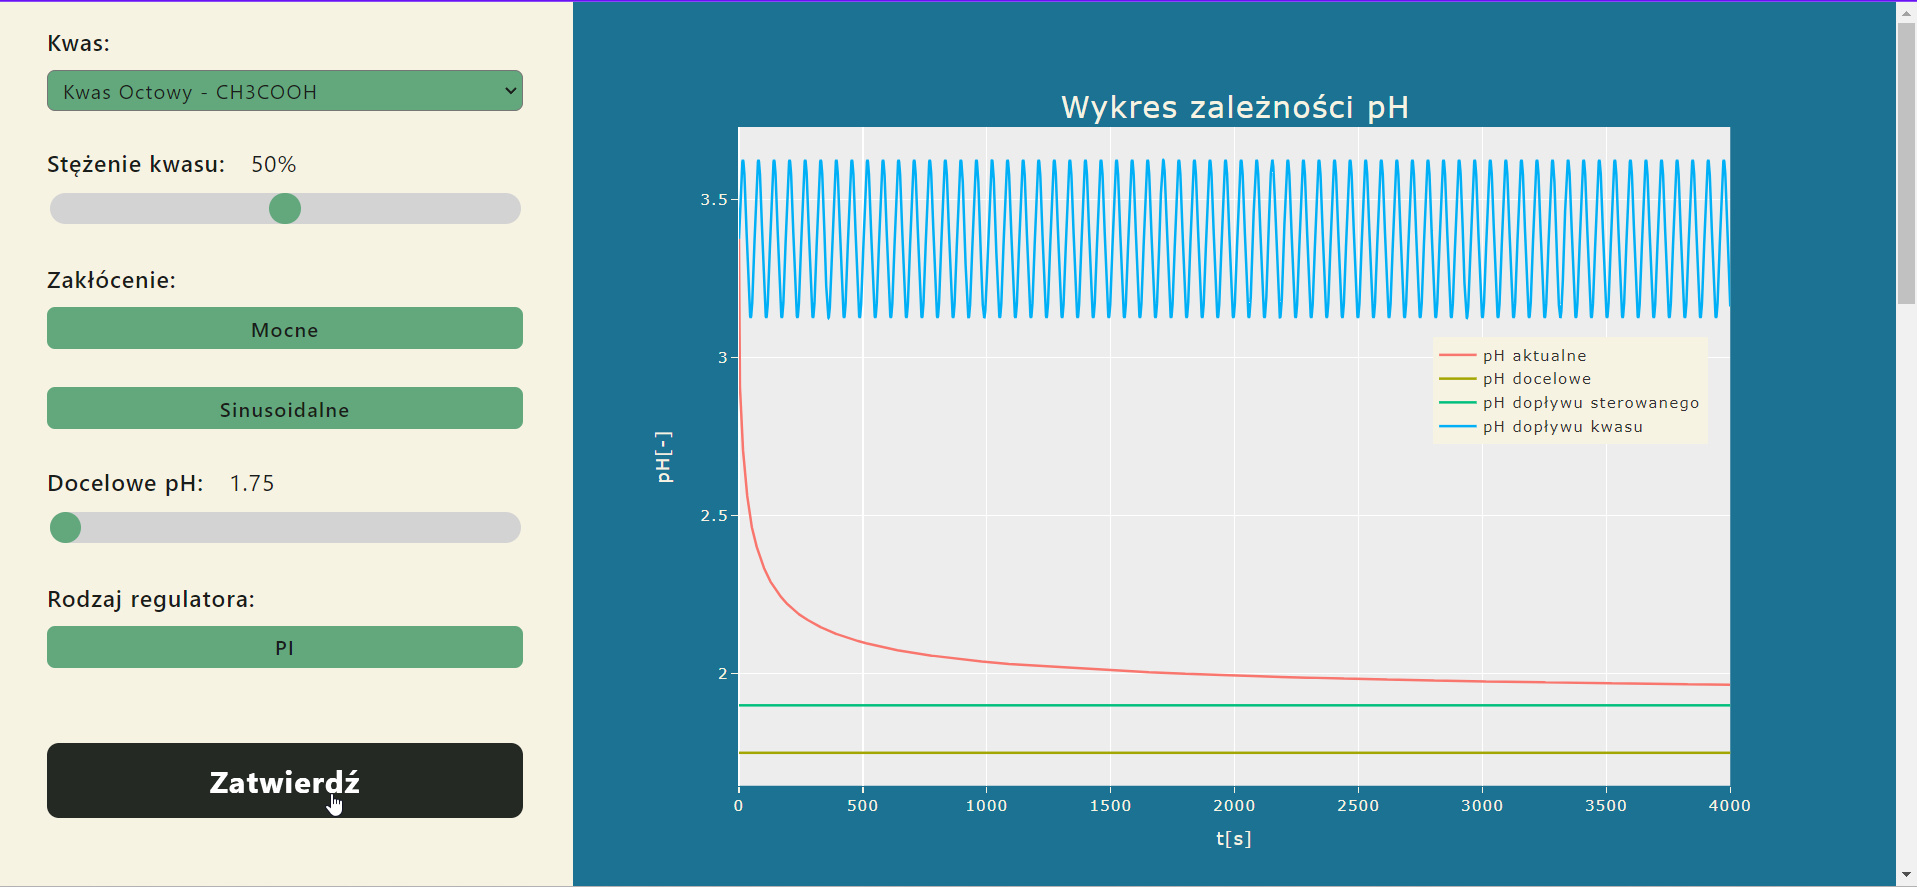
\includegraphics[scale=0.4]{octowy_50_1_75}
	\end{center}
	\newpage
	\begin{center}
		\textbf{Kolejne dwa wykresy obrazują przypadek, gdy docelowe pH znajduje się poza zakresem tworzonym przez pH dopływu sterowanego oraz zakłócenia i nie może być osiągnięte.}\\
		\hspace{0em}\\
		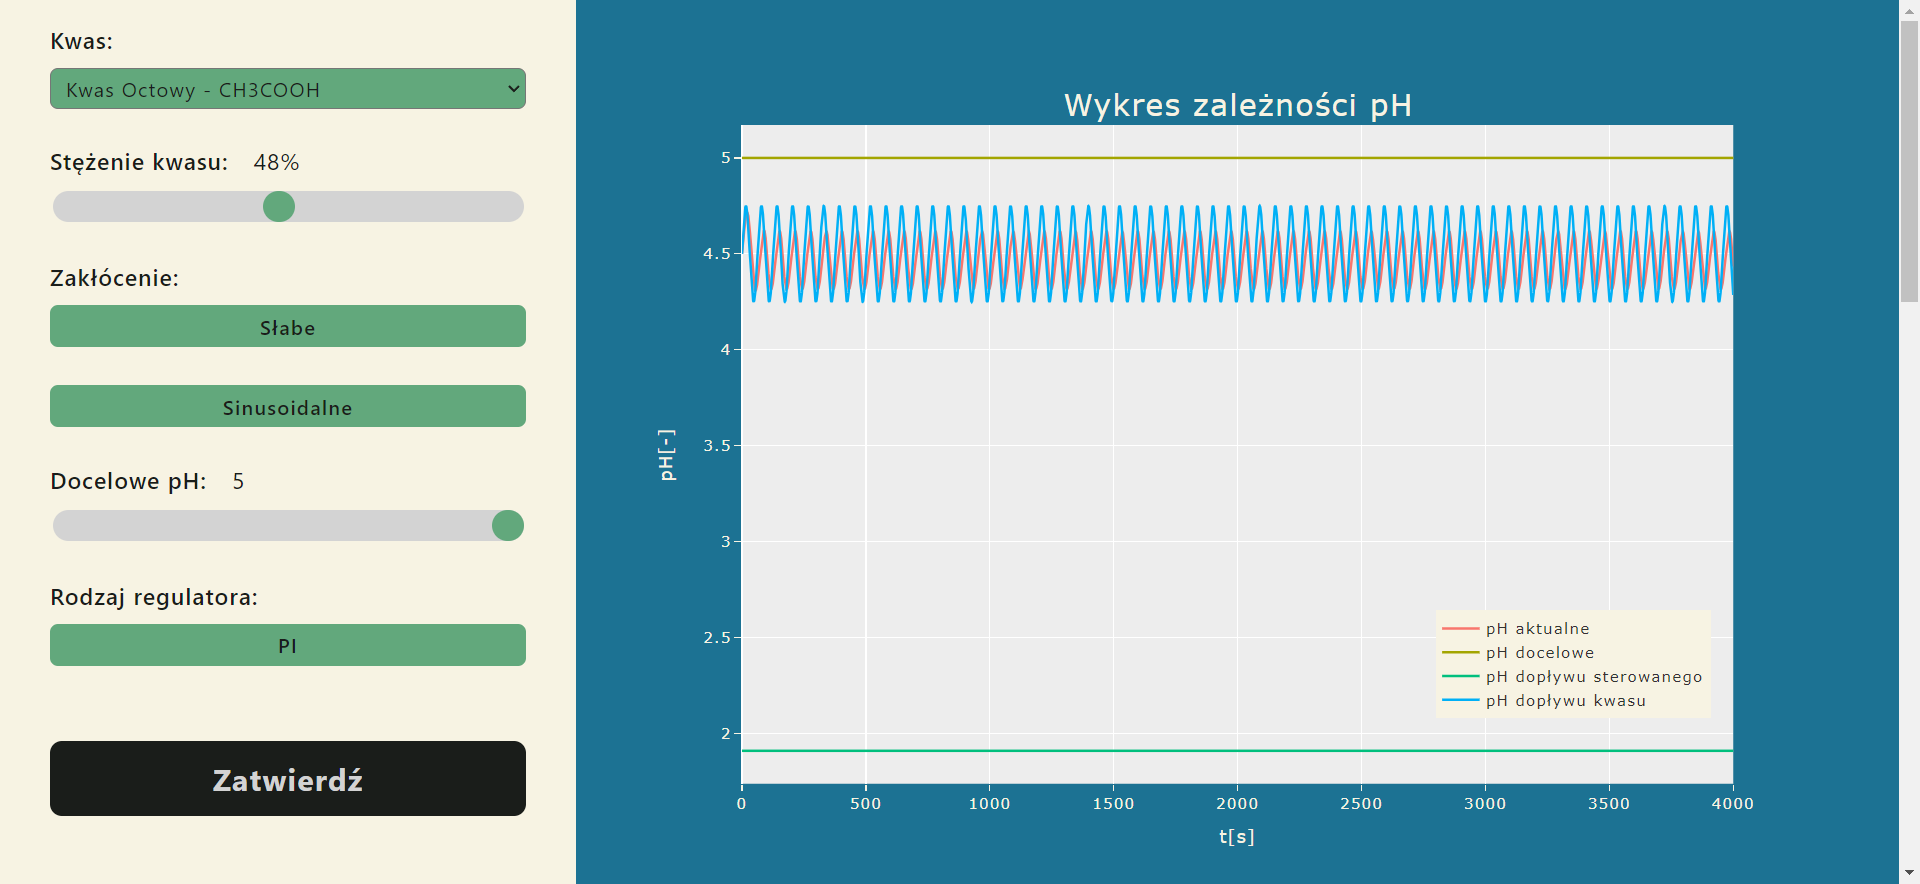
\includegraphics[scale=0.4]{octowy_48_5}\\
		\hspace{0em}\\
		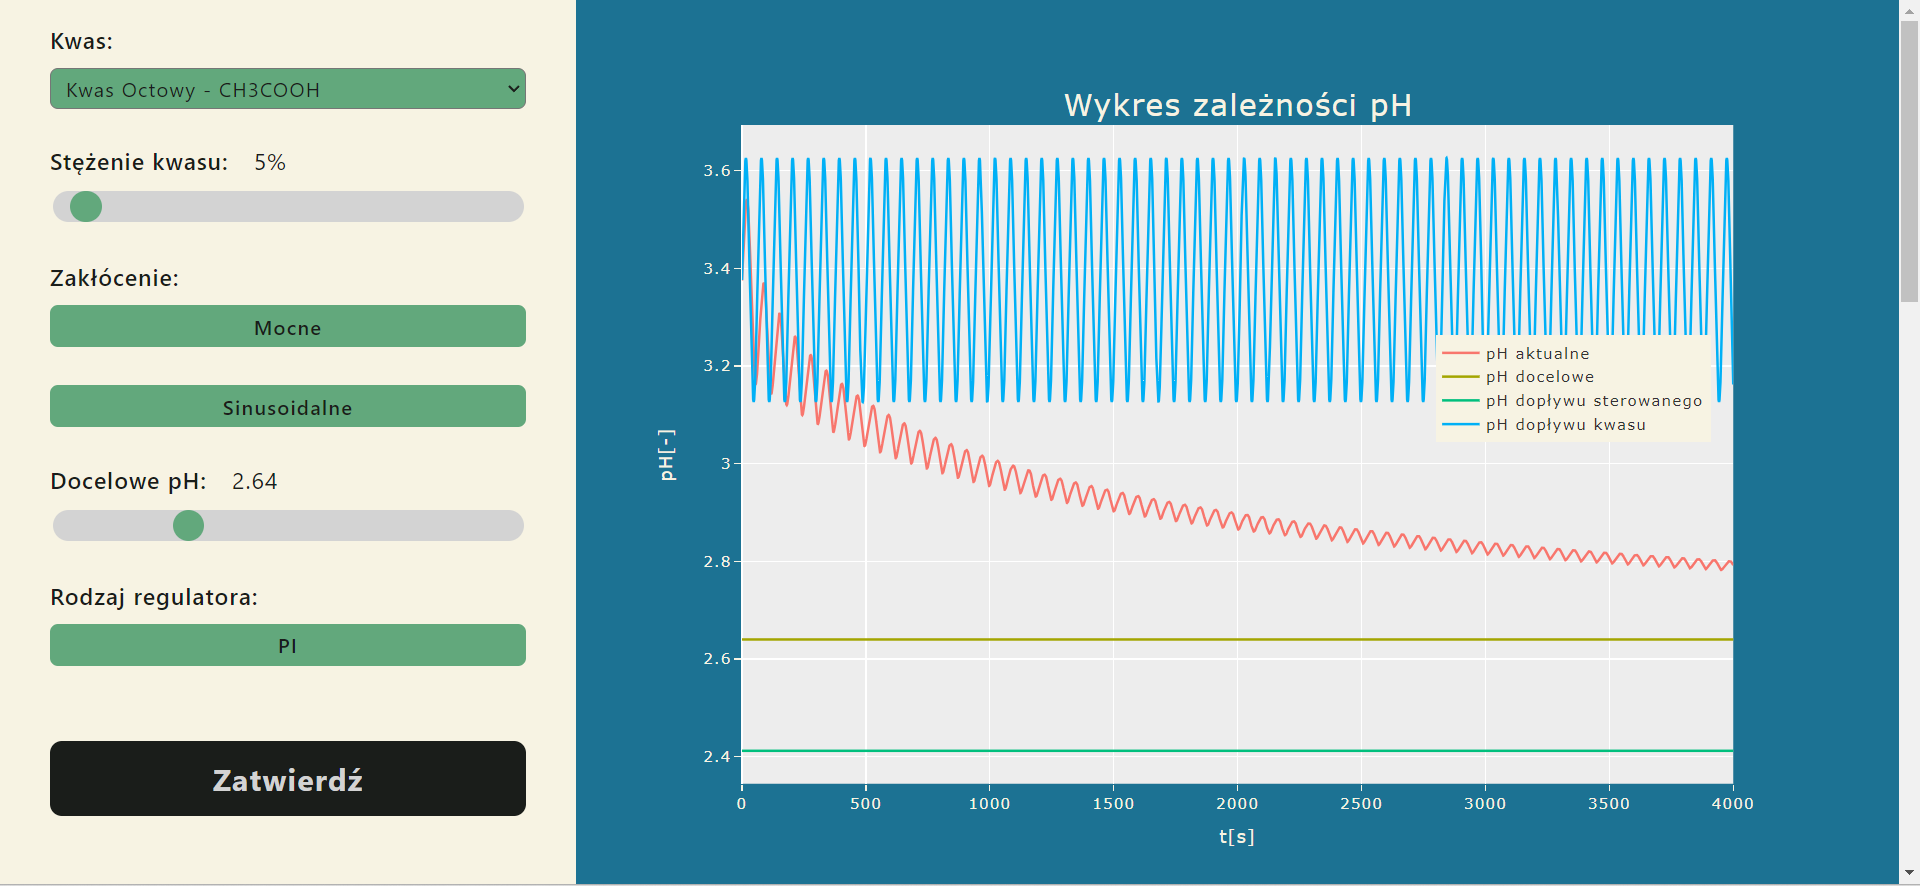
\includegraphics[scale=0.4]{octowy_5_2_64}
	\end{center}
	\newpage
	\begin{center}
		\textbf{Następny wykres przedstawia wyniki dla zastosowania regulatora typu PID zamiast, jak w poprzednich przykładach, PI.}\\
		\hspace{0em}\\
		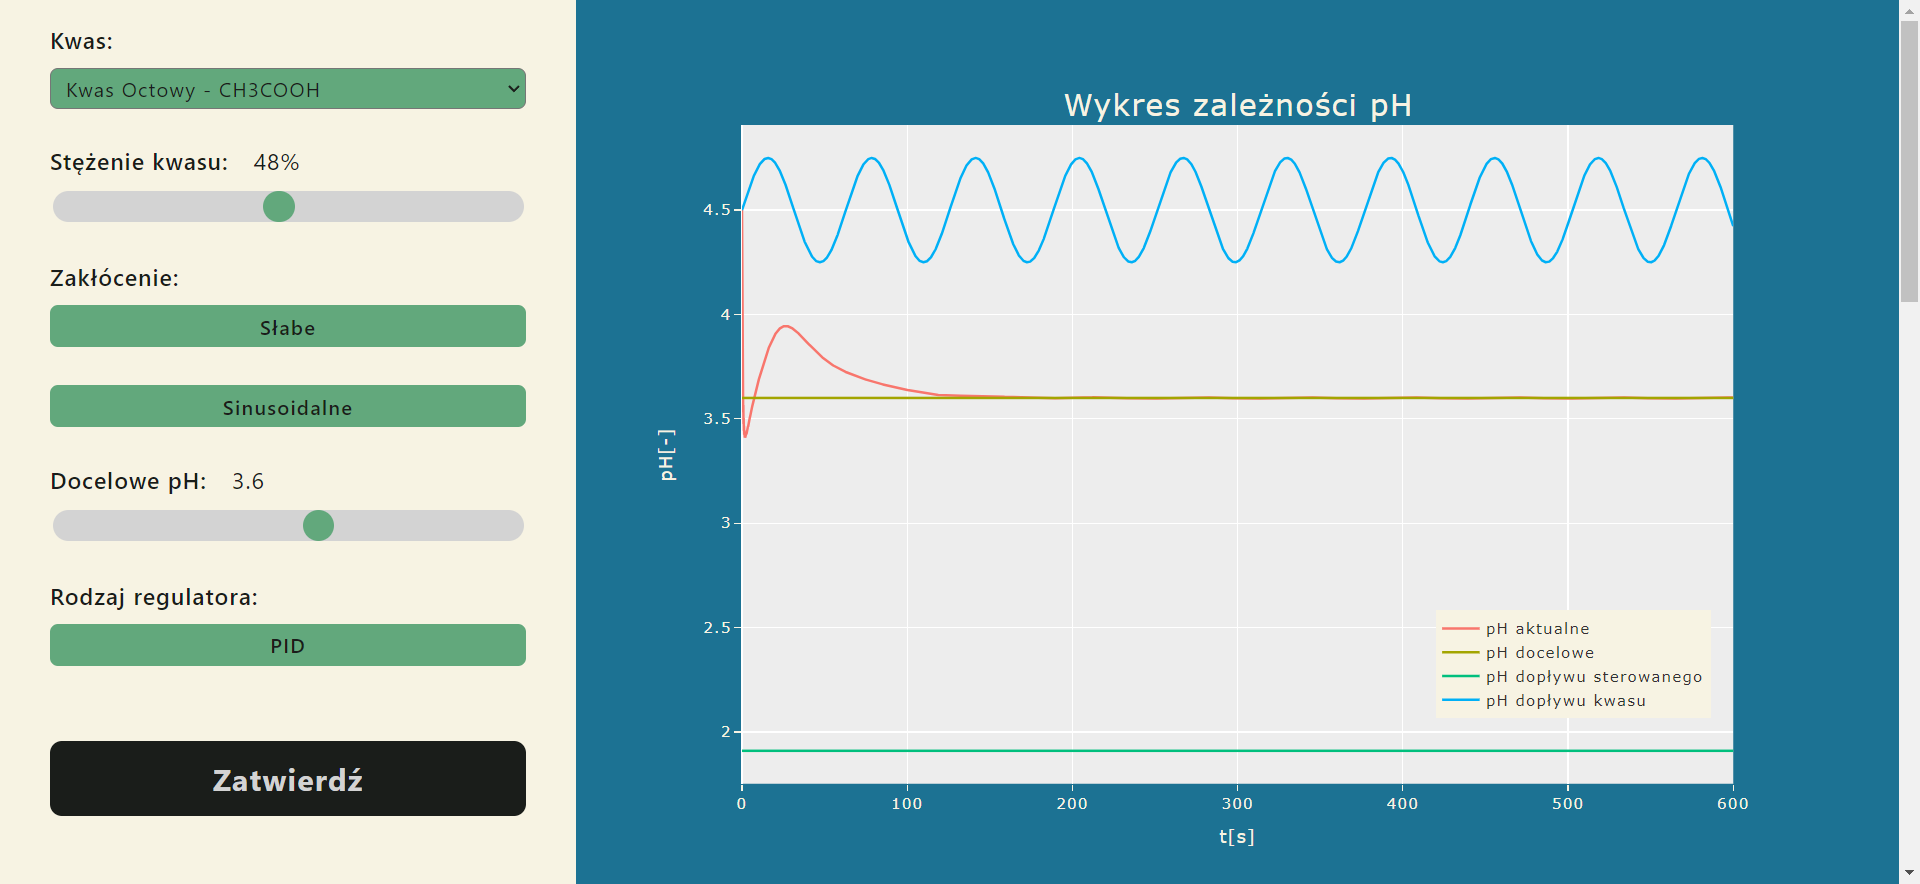
\includegraphics[scale=0.4]{octowy_48_3_6_pid}
	\end{center}
	\begin{center}
		\textbf{Następnie pokazane są wykresy dla trzech innych kwasów z wybraną kombinacją ustawień.}\\
		\hspace{0em}\\
		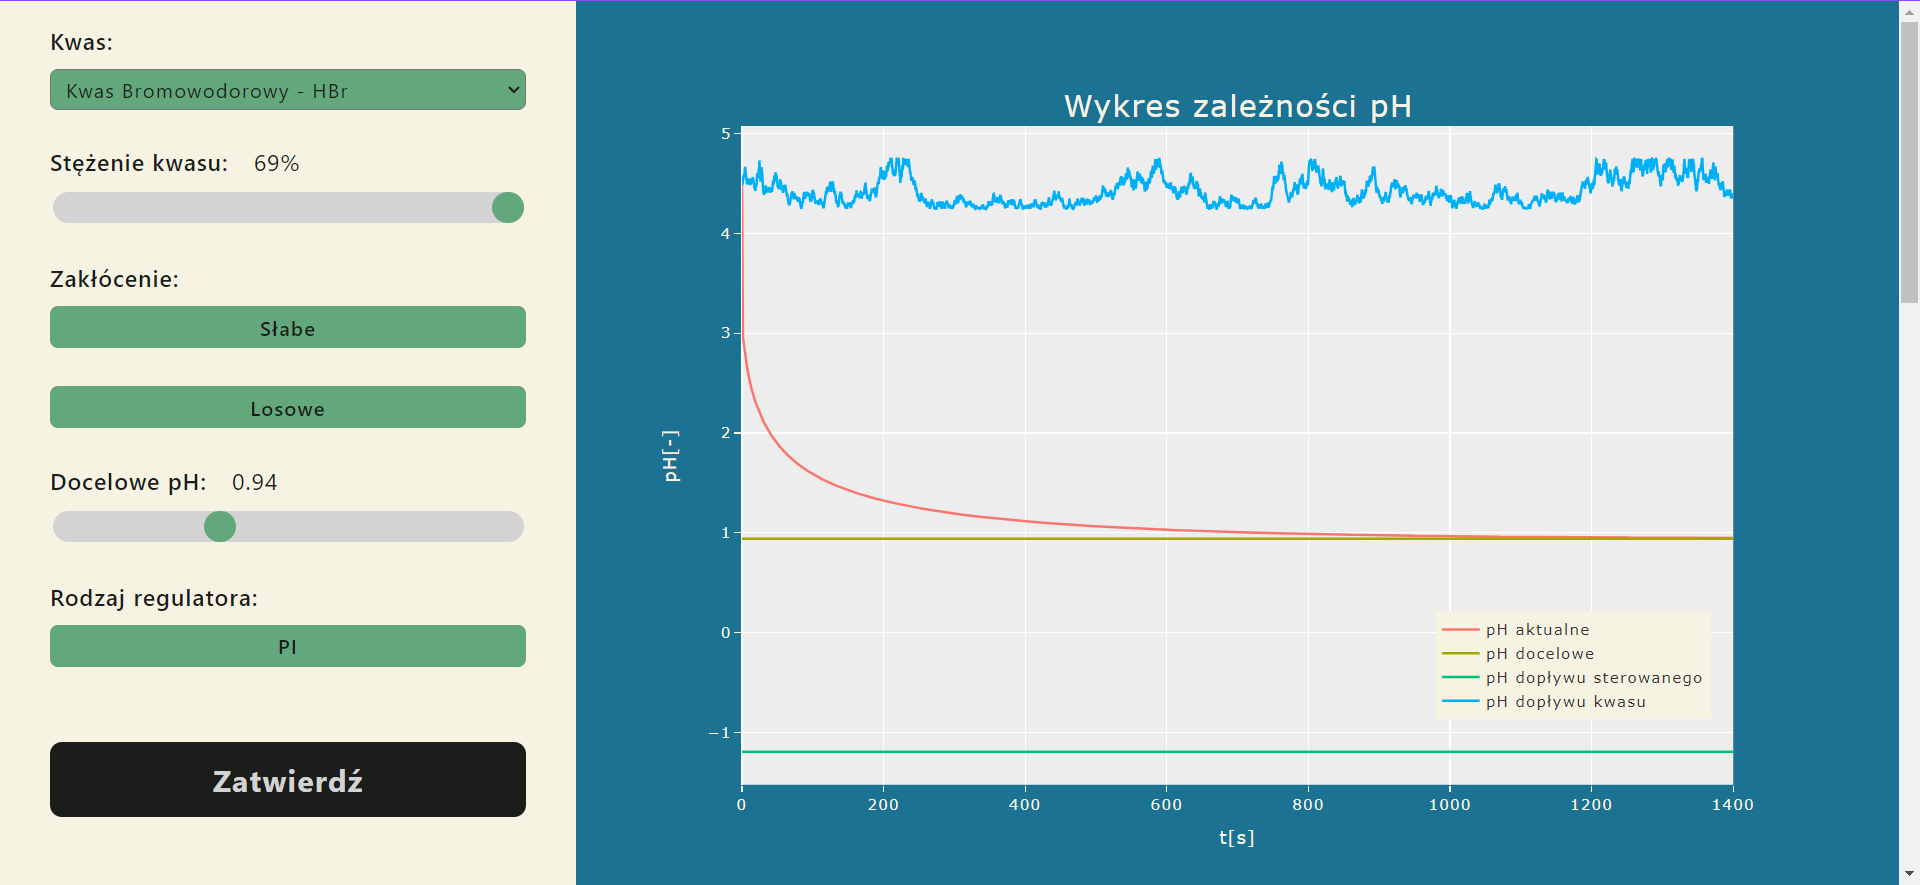
\includegraphics[scale=0.4]{bromowodorowy_69_0_94}
		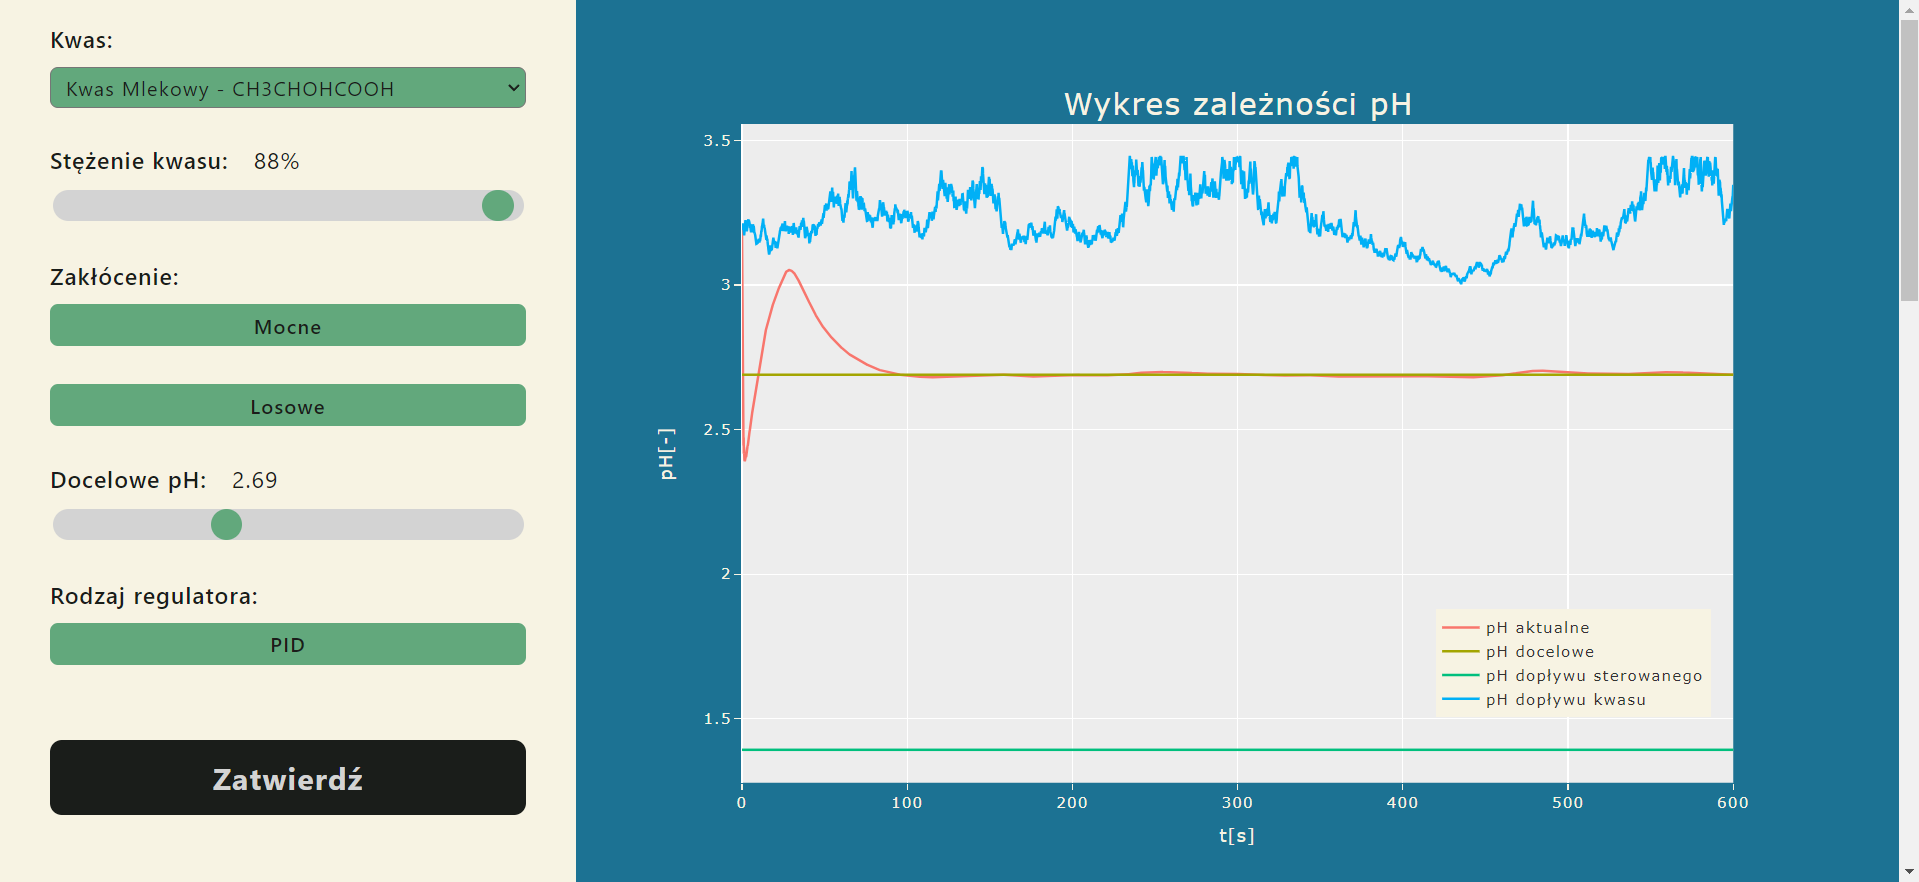
\includegraphics[scale=0.4]{mlekowy_88_2_69}\\
		\hspace{0em}\\
		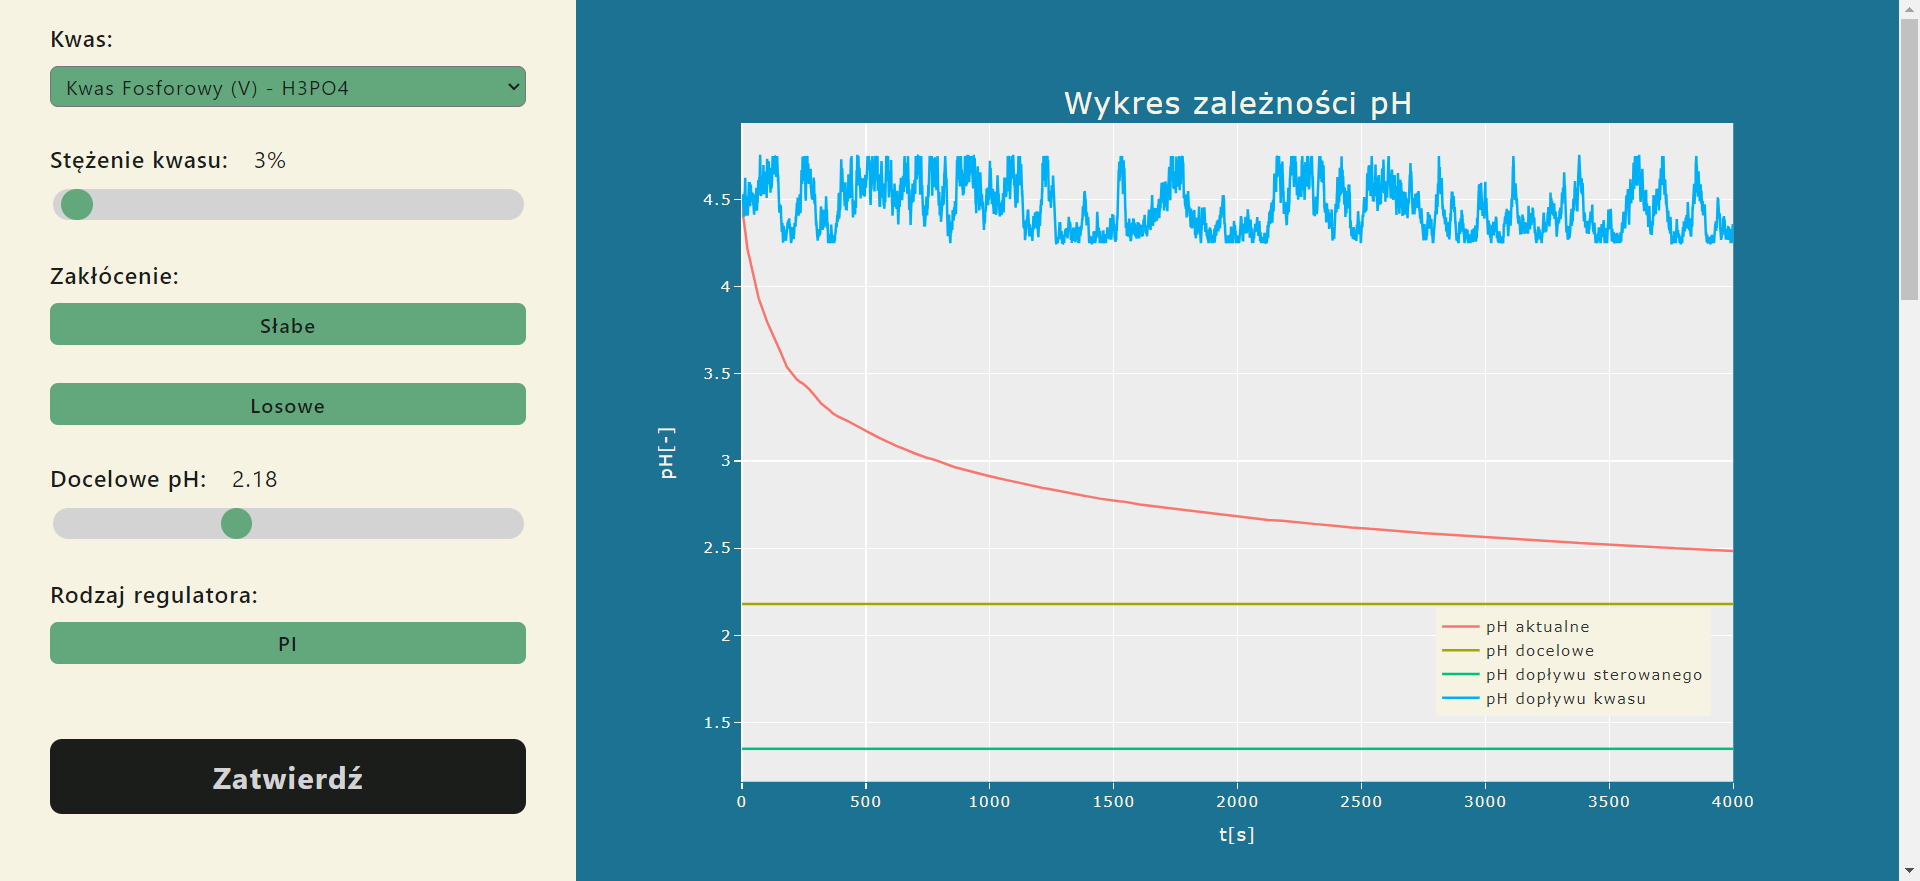
\includegraphics[scale=0.4]{fosforowy}
	\end{center}
	
\end{document}